\subsection{Análisis energético de sistema no conservativo}
    En la sección \ref{caso1}, se observa que el sistema se comporta de la manera 
    esperada ya  que al no existir la influencia de fuerzas exógenas $\boldsymbol{\tau}$ y considerando el efecto de las fuerzas 
    disipativas $\boldsymbol{\tau}_D$, se visualiza en la gráfica de energía mecánica una tendencia de la energía hacia cero, 
    indicando que toda la energía potencial presente en el estado inicial del robot se pierde conforme las articulaciones se mueven, 
    hasta llegar a un estado de reposo. 
    
    Considerando la sección \ref{caso2}, se observa que el sistema se comporta nuevamente como lo esperado, esto debido que 
    al aplicarse fuerzas exógenas $\boldsymbol{\tau}$ ocurre un aumento en la energía mecánica del sistema, transformándose así en 
    energía cinética para el movimiento de cada eslabón. 

    Esto además, permite definir que el torque aplicado a cada grado de libertad supera la fricción viscosa de la articulación, 
    haciendo que las coordenadas generalizadas $\boldsymbol{q}$ cambien de posición en función de la regla de la mano
    derecha.  

\subsection{Análisis energético de sistema conservativo}
    Si se realiza un análisis del caso de la sección \ref{caso3}, 
    se obtienen las Figuras \ref{fig:ec3} y \ref{fig:ep3}
    en un tiempo de $0$ a $5$ $[s]$ donde se representa el comportamiento 
    \emph{complementario} entre la energía cinética con la energía 
    potencial, con el fin de describir una energía mecánica constante. 
    
    \begin{figure}[H]
        \centering
        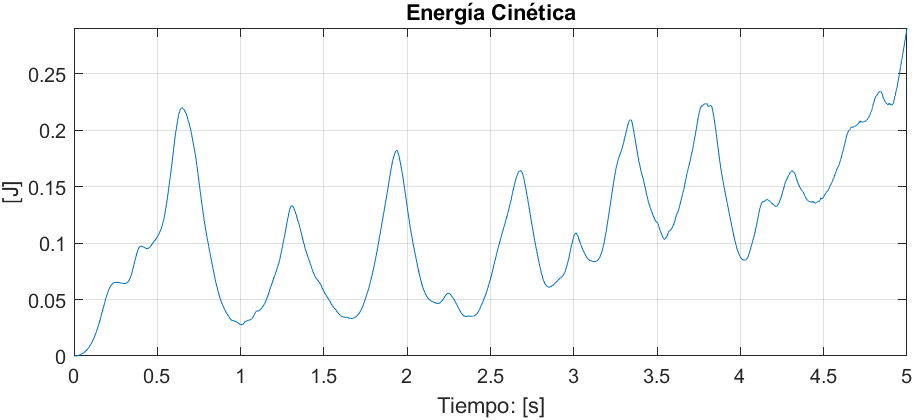
\includegraphics[scale=0.5]{Resultados/ener_cin_caso3_5s.png} 
        \caption{Energía cinética de caso 3, periodo de 5s.}
        \label{fig:ec3}
    \end{figure}

    \begin{figure}[H]
        \centering
        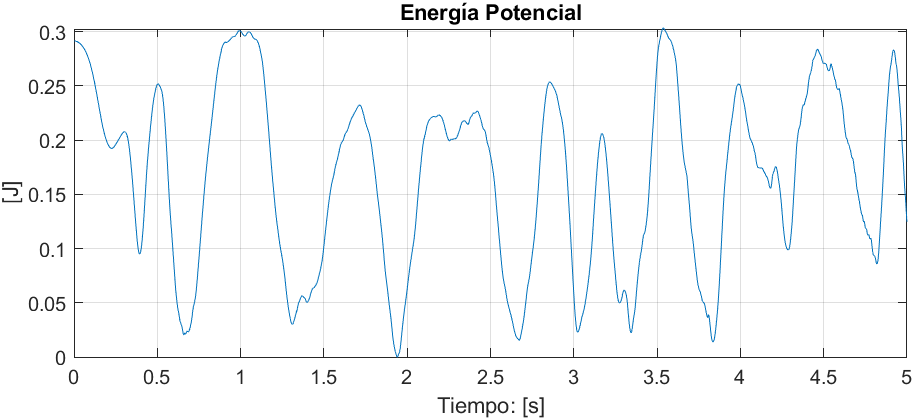
\includegraphics[scale=0.5]{Resultados/ener_pot_caso3_5s.png} 
        \caption{Energía potencial de caso 3, periodo de 5s.}
        \label{fig:ep3}
    \end{figure}

    Sin embargo, puede notarse un aumento en la energía cinética en los últimos segundos, 
    tal como se presenta en la Figura \ref{fig:eCinC3}. Esto es 
    incongruente con los resultados esperados dado que el sistema no puede tener mayor 
    energía cinética que la energía potencial máxima, puesto que no se aplica ninguna 
    fuerza exógena.

    % Punto 3
    Como tercer punto, asumiendo que los resultados incongruentes obtenidos para el 
    último caso de análisis energético son consecuencia del uso de un integrador 
    no adecuado para el tipo de sistema, se procedió a ejecutar el simulador 
    definiendo el integrador de paso fijo \emph{ode3} con un tamaño de paso de 
    0.00001s, esperando obtener una representación congruente con respecto a 
    la conservación de la energía.

    La gráfica de la energía mecánica resultante para un tiempo de $5[s]$ de simulación 
    se presenta en la figura \ref{fig:em_3_ode3}, y se observa que al compararse con la gráfica 
    de energía mecánica haciendo uso del integrador \emph{ode15s} en la figura \ref{fig:em_3}, ambas gráficas presentan 
    comportamientos similares, tanto en sus rangos de amplitud como en los valores que toman 
    en cada instante de tiempo.

    \begin{figure}[H]
        \centering
        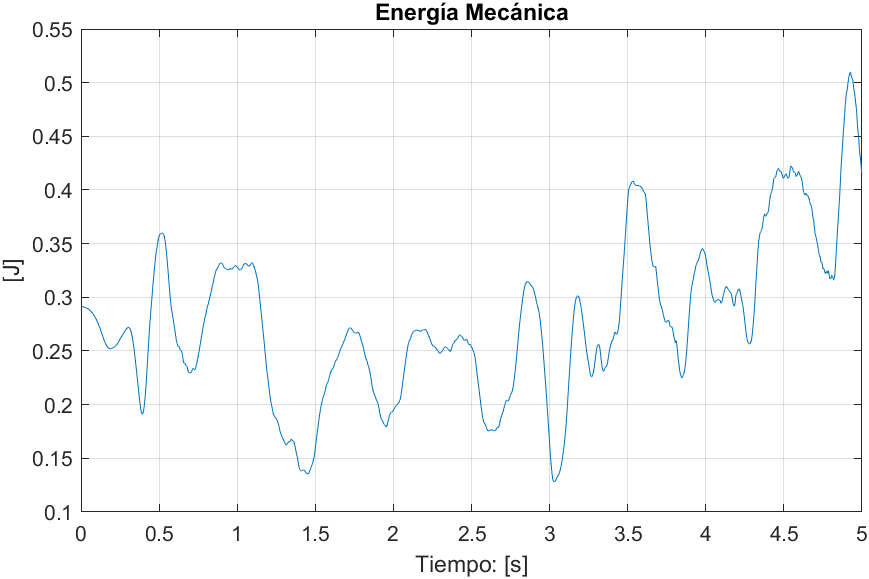
\includegraphics[scale=0.5]{Resultados/ener_mec_caso3_5s.png} 
        \caption{Energía mecánica de caso 3, periodo de 5s.}
        \label{fig:em_3}
    \end{figure}

    \begin{figure}[H]
        \centering
        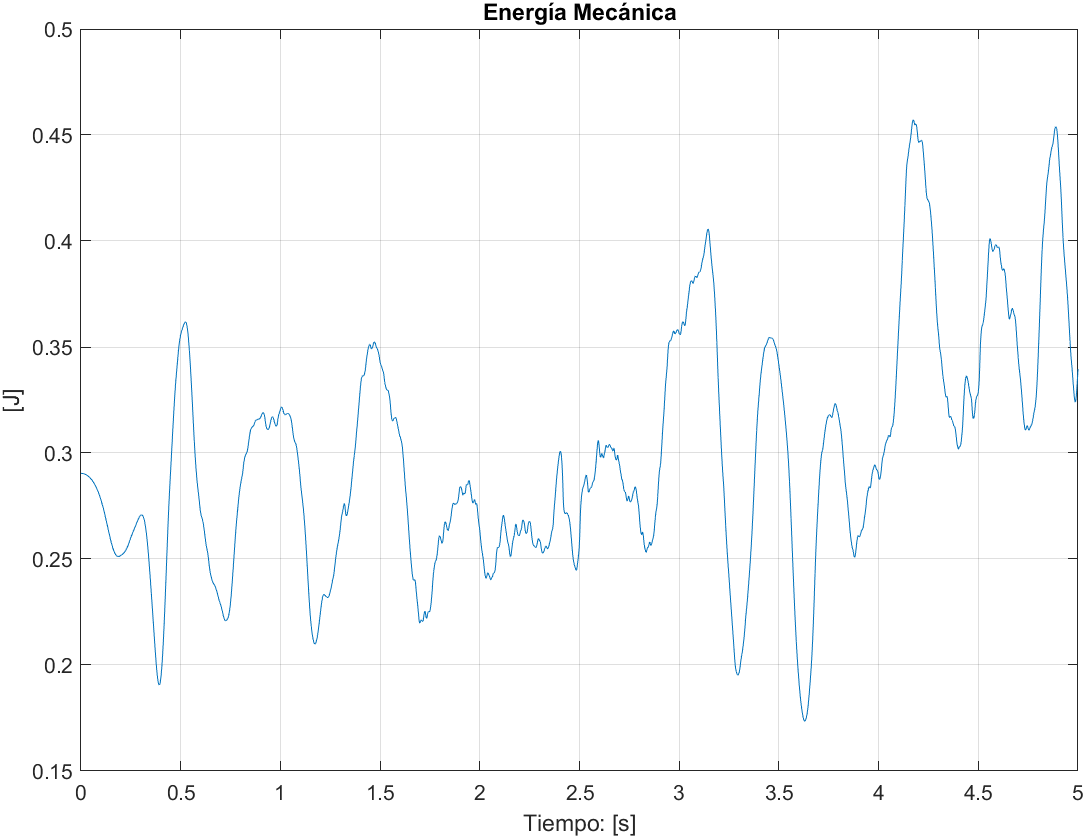
\includegraphics[scale=0.38]{Resultados/ener_mec_caso3_ode3_5s.png} 
        \caption{Energía mecánica de caso 3, periodo de 5s, integrador ode3.}
        \label{fig:em_3_ode3}
    \end{figure}

    De esta manera, se observa una diferencia entre los resultados obtenidos por cualquiera de los integradores con respecto a 
    los resultados esperados. Esta discrepancia puede atribuirse al hecho de que cualquier integrador basado 
    en métodos numéricos que dé solución al modelo dinámico, acumula un error si el tiempo de 
    muestreo utilizado no corresponde con la velocidad de la dinámica del sistema. Es decir, 
    considerando que las gráficas de velocidades generalizadas muestran que el eslabón asociado a $q_6$ 
    incrementa su velocidad en una escala mayor que la del resto de los eslabones, es posible 
    que la frecuencia de oscilación de dicho eslabón sea mayor que la frecuencia de muestreo del integrador 
    y por lo tanto, el causante del fallo en el proceso de integración.

\subsection{Trabajo futuro}
    Se contempla el desarrollo de un segundo simulador basado en 
    la teoría del Acercamiento de Descomposición de Cuerpos (BDA), con el 
    fin de comparar los resultados obtenidos por este simulador.
    
    El cambio de paradigma debería permitir mejorar los tiempos de ejecución, así 
    como reducir el error numérico, verificando si la causa del error para el caso 
    conservativo es debido a la naturaleza del integrador o por la estructura del 
    modelo dinámico actual.

    De igual manera, se analizará el comportamiento del sistema con diferentes métodos 
    de integración, con el objetivo de determinar el más adecuado. 



